% Options for packages loaded elsewhere
\PassOptionsToPackage{unicode}{hyperref}
\PassOptionsToPackage{hyphens}{url}
\PassOptionsToPackage{dvipsnames,svgnames,x11names}{xcolor}
%
\documentclass[
]{article}

\usepackage{amsmath,amssymb}
\usepackage{lmodern}
\usepackage{iftex}
\ifPDFTeX
  \usepackage[T1]{fontenc}
  \usepackage[utf8]{inputenc}
  \usepackage{textcomp} % provide euro and other symbols
\else % if luatex or xetex
  \usepackage{unicode-math}
  \defaultfontfeatures{Scale=MatchLowercase}
  \defaultfontfeatures[\rmfamily]{Ligatures=TeX,Scale=1}
\fi
% Use upquote if available, for straight quotes in verbatim environments
\IfFileExists{upquote.sty}{\usepackage{upquote}}{}
\IfFileExists{microtype.sty}{% use microtype if available
  \usepackage[]{microtype}
  \UseMicrotypeSet[protrusion]{basicmath} % disable protrusion for tt fonts
}{}
\makeatletter
\@ifundefined{KOMAClassName}{% if non-KOMA class
  \IfFileExists{parskip.sty}{%
    \usepackage{parskip}
  }{% else
    \setlength{\parindent}{0pt}
    \setlength{\parskip}{6pt plus 2pt minus 1pt}}
}{% if KOMA class
  \KOMAoptions{parskip=half}}
\makeatother
\usepackage{xcolor}
\setlength{\emergencystretch}{3em} % prevent overfull lines
\setcounter{secnumdepth}{-\maxdimen} % remove section numbering
% Make \paragraph and \subparagraph free-standing
\ifx\paragraph\undefined\else
  \let\oldparagraph\paragraph
  \renewcommand{\paragraph}[1]{\oldparagraph{#1}\mbox{}}
\fi
\ifx\subparagraph\undefined\else
  \let\oldsubparagraph\subparagraph
  \renewcommand{\subparagraph}[1]{\oldsubparagraph{#1}\mbox{}}
\fi

\usepackage{color}
\usepackage{fancyvrb}
\newcommand{\VerbBar}{|}
\newcommand{\VERB}{\Verb[commandchars=\\\{\}]}
\DefineVerbatimEnvironment{Highlighting}{Verbatim}{commandchars=\\\{\}}
% Add ',fontsize=\small' for more characters per line
\usepackage{framed}
\definecolor{shadecolor}{RGB}{241,243,245}
\newenvironment{Shaded}{\begin{snugshade}}{\end{snugshade}}
\newcommand{\AlertTok}[1]{\textcolor[rgb]{0.68,0.00,0.00}{#1}}
\newcommand{\AnnotationTok}[1]{\textcolor[rgb]{0.37,0.37,0.37}{#1}}
\newcommand{\AttributeTok}[1]{\textcolor[rgb]{0.40,0.45,0.13}{#1}}
\newcommand{\BaseNTok}[1]{\textcolor[rgb]{0.68,0.00,0.00}{#1}}
\newcommand{\BuiltInTok}[1]{\textcolor[rgb]{0.00,0.23,0.31}{#1}}
\newcommand{\CharTok}[1]{\textcolor[rgb]{0.13,0.47,0.30}{#1}}
\newcommand{\CommentTok}[1]{\textcolor[rgb]{0.37,0.37,0.37}{#1}}
\newcommand{\CommentVarTok}[1]{\textcolor[rgb]{0.37,0.37,0.37}{\textit{#1}}}
\newcommand{\ConstantTok}[1]{\textcolor[rgb]{0.56,0.35,0.01}{#1}}
\newcommand{\ControlFlowTok}[1]{\textcolor[rgb]{0.00,0.23,0.31}{#1}}
\newcommand{\DataTypeTok}[1]{\textcolor[rgb]{0.68,0.00,0.00}{#1}}
\newcommand{\DecValTok}[1]{\textcolor[rgb]{0.68,0.00,0.00}{#1}}
\newcommand{\DocumentationTok}[1]{\textcolor[rgb]{0.37,0.37,0.37}{\textit{#1}}}
\newcommand{\ErrorTok}[1]{\textcolor[rgb]{0.68,0.00,0.00}{#1}}
\newcommand{\ExtensionTok}[1]{\textcolor[rgb]{0.00,0.23,0.31}{#1}}
\newcommand{\FloatTok}[1]{\textcolor[rgb]{0.68,0.00,0.00}{#1}}
\newcommand{\FunctionTok}[1]{\textcolor[rgb]{0.28,0.35,0.67}{#1}}
\newcommand{\ImportTok}[1]{\textcolor[rgb]{0.00,0.46,0.62}{#1}}
\newcommand{\InformationTok}[1]{\textcolor[rgb]{0.37,0.37,0.37}{#1}}
\newcommand{\KeywordTok}[1]{\textcolor[rgb]{0.00,0.23,0.31}{#1}}
\newcommand{\NormalTok}[1]{\textcolor[rgb]{0.00,0.23,0.31}{#1}}
\newcommand{\OperatorTok}[1]{\textcolor[rgb]{0.37,0.37,0.37}{#1}}
\newcommand{\OtherTok}[1]{\textcolor[rgb]{0.00,0.23,0.31}{#1}}
\newcommand{\PreprocessorTok}[1]{\textcolor[rgb]{0.68,0.00,0.00}{#1}}
\newcommand{\RegionMarkerTok}[1]{\textcolor[rgb]{0.00,0.23,0.31}{#1}}
\newcommand{\SpecialCharTok}[1]{\textcolor[rgb]{0.37,0.37,0.37}{#1}}
\newcommand{\SpecialStringTok}[1]{\textcolor[rgb]{0.13,0.47,0.30}{#1}}
\newcommand{\StringTok}[1]{\textcolor[rgb]{0.13,0.47,0.30}{#1}}
\newcommand{\VariableTok}[1]{\textcolor[rgb]{0.07,0.07,0.07}{#1}}
\newcommand{\VerbatimStringTok}[1]{\textcolor[rgb]{0.13,0.47,0.30}{#1}}
\newcommand{\WarningTok}[1]{\textcolor[rgb]{0.37,0.37,0.37}{\textit{#1}}}

\providecommand{\tightlist}{%
  \setlength{\itemsep}{0pt}\setlength{\parskip}{0pt}}\usepackage{longtable,booktabs,array}
\usepackage{calc} % for calculating minipage widths
% Correct order of tables after \paragraph or \subparagraph
\usepackage{etoolbox}
\makeatletter
\patchcmd\longtable{\par}{\if@noskipsec\mbox{}\fi\par}{}{}
\makeatother
% Allow footnotes in longtable head/foot
\IfFileExists{footnotehyper.sty}{\usepackage{footnotehyper}}{\usepackage{footnote}}
\makesavenoteenv{longtable}
\usepackage{graphicx}
\makeatletter
\def\maxwidth{\ifdim\Gin@nat@width>\linewidth\linewidth\else\Gin@nat@width\fi}
\def\maxheight{\ifdim\Gin@nat@height>\textheight\textheight\else\Gin@nat@height\fi}
\makeatother
% Scale images if necessary, so that they will not overflow the page
% margins by default, and it is still possible to overwrite the defaults
% using explicit options in \includegraphics[width, height, ...]{}
\setkeys{Gin}{width=\maxwidth,height=\maxheight,keepaspectratio}
% Set default figure placement to htbp
\makeatletter
\def\fps@figure{htbp}
\makeatother
\newlength{\cslhangindent}
\setlength{\cslhangindent}{1.5em}
\newlength{\csllabelwidth}
\setlength{\csllabelwidth}{3em}
\newlength{\cslentryspacingunit} % times entry-spacing
\setlength{\cslentryspacingunit}{\parskip}
\newenvironment{CSLReferences}[2] % #1 hanging-ident, #2 entry spacing
 {% don't indent paragraphs
  \setlength{\parindent}{0pt}
  % turn on hanging indent if param 1 is 1
  \ifodd #1
  \let\oldpar\par
  \def\par{\hangindent=\cslhangindent\oldpar}
  \fi
  % set entry spacing
  \setlength{\parskip}{#2\cslentryspacingunit}
 }%
 {}
\usepackage{calc}
\newcommand{\CSLBlock}[1]{#1\hfill\break}
\newcommand{\CSLLeftMargin}[1]{\parbox[t]{\csllabelwidth}{#1}}
\newcommand{\CSLRightInline}[1]{\parbox[t]{\linewidth - \csllabelwidth}{#1}\break}
\newcommand{\CSLIndent}[1]{\hspace{\cslhangindent}#1}

\usepackage{booktabs}
\usepackage{longtable}
\usepackage{array}
\usepackage{multirow}
\usepackage{wrapfig}
\usepackage{float}
\usepackage{colortbl}
\usepackage{pdflscape}
\usepackage{tabu}
\usepackage{threeparttable}
\usepackage{threeparttablex}
\usepackage[normalem]{ulem}
\usepackage{makecell}
\usepackage{xcolor}
\usepackage[noblocks]{authblk}
\renewcommand*{\Authsep}{, }
\renewcommand*{\Authand}{, }
\renewcommand*{\Authands}{, }
\renewcommand\Affilfont{\small}
\makeatletter
\makeatother
\makeatletter
\makeatother
\makeatletter
\@ifpackageloaded{caption}{}{\usepackage{caption}}
\AtBeginDocument{%
\ifdefined\contentsname
  \renewcommand*\contentsname{Table of contents}
\else
  \newcommand\contentsname{Table of contents}
\fi
\ifdefined\listfigurename
  \renewcommand*\listfigurename{List of Figures}
\else
  \newcommand\listfigurename{List of Figures}
\fi
\ifdefined\listtablename
  \renewcommand*\listtablename{List of Tables}
\else
  \newcommand\listtablename{List of Tables}
\fi
\ifdefined\figurename
  \renewcommand*\figurename{Figure}
\else
  \newcommand\figurename{Figure}
\fi
\ifdefined\tablename
  \renewcommand*\tablename{Table}
\else
  \newcommand\tablename{Table}
\fi
}
\@ifpackageloaded{float}{}{\usepackage{float}}
\floatstyle{ruled}
\@ifundefined{c@chapter}{\newfloat{codelisting}{h}{lop}}{\newfloat{codelisting}{h}{lop}[chapter]}
\floatname{codelisting}{Listing}
\newcommand*\listoflistings{\listof{codelisting}{List of Listings}}
\makeatother
\makeatletter
\@ifpackageloaded{caption}{}{\usepackage{caption}}
\@ifpackageloaded{subcaption}{}{\usepackage{subcaption}}
\makeatother
\makeatletter
\@ifpackageloaded{tcolorbox}{}{\usepackage[many]{tcolorbox}}
\makeatother
\makeatletter
\@ifundefined{shadecolor}{\definecolor{shadecolor}{rgb}{.97, .97, .97}}
\makeatother
\makeatletter
\makeatother
\ifLuaTeX
  \usepackage{selnolig}  % disable illegal ligatures
\fi
\IfFileExists{bookmark.sty}{\usepackage{bookmark}}{\usepackage{hyperref}}
\IfFileExists{xurl.sty}{\usepackage{xurl}}{} % add URL line breaks if available
\urlstyle{same} % disable monospaced font for URLs
\hypersetup{
  pdftitle={InfiltrodiscR: an R package for infiltrometer data analysis and an experience for improving data reproducibility in a soil physics laboratory},
  pdfauthor={Carolina V. Giraldo; Sara E. Acevedo},
  colorlinks=true,
  linkcolor={blue},
  filecolor={Maroon},
  citecolor={Blue},
  urlcolor={Blue},
  pdfcreator={LaTeX via pandoc}}

\title{InfiltrodiscR: an R package for infiltrometer data analysis and
an experience for improving data reproducibility in a soil physics
laboratory}


\author[1]{Carolina V. Giraldo}
\author[1,2]{Sara E. Acevedo}

\affil[1]{Pontificia Universidad Católica de Chile}
\affil[2]{Centro de Desarrollo Urbano Sustentable (CEDEUS)}


\date{}
\begin{document}
\maketitle
\ifdefined\Shaded\renewenvironment{Shaded}{\begin{tcolorbox}[interior hidden, enhanced, borderline west={3pt}{0pt}{shadecolor}, sharp corners, breakable, boxrule=0pt, frame hidden]}{\end{tcolorbox}}\fi

\hypertarget{abstract}{%
\subsection{Abstract}\label{abstract}}

This paper addresses the increasing interest and knowledge among soil
physics researchers to use R, language which offers distinct advantages
in terms of data reproducibility. Achieving reproducibility is a
challenge in various scientific fields, including soil science, and is
further driven by the demand for transparency from funding agencies and
governmental institutions. Open and reproducible soil physics research
can have significant positive impacts on the scientific community.
Motivated by the goal of promoting open and equitable research, the
authors leveraged the existing knowledge of R in a soil physics
laboratory (Soil Biophysics Laboratory) and the need for a repository
with common functions for infiltrometer data analysis, developed the R
package infiltrodiscR. The goal of infiltrodiscR is to provide functions
for the fitting of data derived from the Minidisk Infiltrometer device.

\hypertarget{introduction}{%
\subsection{Introduction}\label{introduction}}

Many soil physics researchers are unacquainted about the functionalities
of the programing language R (Sousa et al. 2020). R is a is a
programming language primarily used for statistical and data analysis.
One main functionality that differentiates R from spreadsheet-based
programs is that R scripts are text-based, making them easily shareable
and reproducible, allowing to replicate analyses. The challenge of
achieving reproducibility persists across various scientific
disciplines, extending it to soil science as well (Correndo et al.
2023). Also, researchers in soil science, and almost every other field,
are being pushed by funding agencies and governmental institutions to
increase transparency and reproducibility of their work (Bond-Lamberty,
Smith, and Bailey 2016). Open, accessible, reusable, and reproducible
soil hydrologic research can have a significant positive impact on the
scientific community and broader society (Hall et al. 2022). In this
work, an R package (infiltrodiscR) is presented containing R functions
compatible with tidyverse package for infiltrometer data analysis.

\hypertarget{motivation}{%
\subsection{Motivation}\label{motivation}}

In 2023, the authors of this work joined to a program lead by Open Life
Science; a community-oriented non-profit organisation that promotes
open, inclusive and equitable research (Haynes 2023). In addition, the
members of the Soil Biophysics laboratory (Soil Biophysics Lab 2023)
already had knowledge of R but there was no repository with common
functions for the infiltrometer data analysis. Based on the programming
expertise of the laboratory members and the need of adoption of open and
reproducible science, the R package InfiltrodiscR was developed (Acevedo
and Giraldo 2023). The goal of infiltrodiscR is to provide functions for
the fitting of data derived from the Minidisk Infiltrometer device. To
determine the unsaturated hydraulic conductivity for a specific suction,
infiltrodiscR uses the relationship between cumulative infiltration
vs.~time. The hydraulic conductivity of the soil (K\textsubscript{(h)})
is calculated as the ratio of C\textsubscript{1}(the slope of the curve
of the cumulative infiltration vs.~the square root of time) and A
(parameter depending on the van Genuchten parameters, the disk radius
and the applied suction) based on the equation proposed by Zhang (1997).

\hypertarget{r-package-description}{%
\subsection{R package description}\label{r-package-description}}

The R package is currently hosted in GitHub. This web-based Git
repository hosting service is currently used by many scientists to work
in teams or collaborative projects (Bond-Lamberty, Smith, and Bailey
2016). Also, the code was deposited in Zenodo, a free service for
hosting data and software that offers long-term (20-year) storage and
integration with GitHub (Hall et al. 2022). The infiltrodiscR package
has a DOI so it can be used as reference in publications and clearly
define the software version used (Acevedo and Giraldo 2023).

To install the R package, the users need to run to following lines:

\begin{Shaded}
\begin{Highlighting}[]
\CommentTok{\# install.packages("devtools")}
\NormalTok{devtools}\SpecialCharTok{::}\FunctionTok{install\_github}\NormalTok{(}\StringTok{"biofisicasuelos/infiltrodiscR"}\NormalTok{)}
\end{Highlighting}
\end{Shaded}

Data needed for running the functions are data stored in \textbf{.csv}
or \textbf{.xlsx} containing columns called as follows:

\begin{itemize}
\tightlist
\item
  texture: soil texture according to USDA: as.character() and lowercase,
  for example ``clay loam''.
\item
  suction: as.character() and lowercase, in this format: ``2cm''. Values
  allowed: ``0.5cm'',``1cm'',``2cm'',``3cm'',``4cm'',``5cm'',``6cm'',
  and ``7cm''.
\item
  volume: volume recorded in the infiltration measurements in mL,
  as.numeric().
\item
  time: time recorded in the infiltration measurements in seconds,
  as.numeric().
\end{itemize}

\newpage{}

\hypertarget{main-functions}{%
\subsection{Main functions:}\label{main-functions}}

\textbf{\texttt{infiltration()}}

This function calculates cumulative infiltration and the square root of
time, using time and volume recorded based on the relationship described
by Philip (1957):

\[I = C_{1} t + C_{2} t^{0.5} \] \textbf{\texttt{vg\_par()}}

This function returns the parameter \emph{A}, \emph{no\_h} and
\emph{alpha} related to the van Genuchten parameters (Genuchten 1980),
from tabulated data calculated for a radius of 2.25 cm, including 12
soil texture classes and suctions from -0.5 cm to -7 cm. Table 1 show
selected data gathered from Meter Group (2023) and Carsel and Parrish
(1988).

\begin{table}

\caption{Table 1. Selected data from the InfiltrodiscR package}
\centering
\begin{tabular}[t]{l|r|r|r|r|r}
\hline
texture & alpha & n/ho & 2cm & 4cm & 6cm\\
\hline
sand & 0.145 & 2.68 & 1.727908 & 0.8926213 & 0.4611201\\
\hline
loamy sand & 0.124 & 2.28 & 2.428600 & 1.8443631 & 1.4006735\\
\hline
sandy loam & 0.075 & 1.89 & 3.909913 & 3.9541483 & 3.9988836\\
\hline
loam & 0.036 & 1.56 & 6.267384 & 7.5304822 & 9.0481388\\
\hline
silt & 0.016 & 1.37 & 8.714378 & 9.8964325 & 11.2388254\\
\hline
silt loam & 0.020 & 1.41 & 7.929874 & 9.1856010 & 10.6401773\\
\hline
sandy clay loam & 0.059 & 1.48 & 4.242925 & 6.1530807 & 8.9231845\\
\hline
clay loam & 0.019 & 1.31 & 6.644845 & 7.8616094 & 9.3011807\\
\hline
silty clay loam & 0.010 & 1.23 & 8.511175 & 9.4110072 & 10.4059732\\
\hline
sandy clay & 0.027 & 1.23 & 4.089288 & 5.3640585 & 7.0362184\\
\hline
silty clay & 0.005 & 1.09 & 6.359575 & 6.7578953 & 7.1811641\\
\hline
clay & 0.008 & 1.09 & 4.300401 & 4.7393888 & 5.2231893\\
\hline
\end{tabular}
\end{table}

\textbf{\texttt{parameter\_A()}}

This function returns the parameter \emph{A} calculated from the
equation based on the work developed by Zhang (1997), where the
parameters \emph{A}, \emph{no\_h} and \emph{alpha} determined previously
are input in the following equations described in Meter Group (2023) and
Surda et al. (2019)

\[A = \frac{11.65(n^{0.1}-1)exp[2.92(n - 1.9)\alpha h_{0}]}{(\alpha r_{0})^{0.91}} ; n\geq 1.9 \]
\[A = \frac{11.65(n^{0.1}-1)exp[7.5(n - 1.9)\alpha h_{0}]}{(\alpha r_{0})^{0.91}} ; n < 1.9 \]

\newpage{}

\hypertarget{practical-example}{%
\subsection{Practical example}\label{practical-example}}

First, some dummy data about infiltration and soils is created. Volume
recorded in the infiltration measurements must be in mL and time in
seconds. Both variables must be numeric. In order to join data
(combining two datasets: infiltration and soil data), a common
identifier or ID column must be present in both datasets. Soil and
infiltration data must have a common column describing each unique soil
and measurement. In this example, a column called soil contains
measurements of ``soil\_a'' and ``soil\_b'' in both datasets

\begin{Shaded}
\begin{Highlighting}[]
\NormalTok{infiltration\_data }\OtherTok{\textless{}{-}} \FunctionTok{tibble}\NormalTok{(}
  \AttributeTok{soil =} \FunctionTok{c}\NormalTok{(}\FunctionTok{rep}\NormalTok{(}\StringTok{"soil\_a"}\NormalTok{,}\DecValTok{11}\NormalTok{), }\FunctionTok{rep}\NormalTok{(}\StringTok{"soil\_b"}\NormalTok{,}\DecValTok{11}\NormalTok{)),}
  \AttributeTok{time =} \FunctionTok{c}\NormalTok{(}\DecValTok{0}\NormalTok{, }\DecValTok{30}\NormalTok{, }\DecValTok{60}\NormalTok{, }\DecValTok{90}\NormalTok{, }\DecValTok{120}\NormalTok{, }\DecValTok{150}\NormalTok{, }\DecValTok{180}\NormalTok{, }\DecValTok{210}\NormalTok{, }\DecValTok{240}\NormalTok{, }\DecValTok{270}\NormalTok{, }\DecValTok{300}\NormalTok{, }\CommentTok{\# seconds}
           \DecValTok{0}\NormalTok{, }\DecValTok{35}\NormalTok{, }\DecValTok{65}\NormalTok{, }\DecValTok{95}\NormalTok{, }\DecValTok{125}\NormalTok{, }\DecValTok{155}\NormalTok{, }\DecValTok{185}\NormalTok{, }\DecValTok{215}\NormalTok{, }\DecValTok{245}\NormalTok{, }\DecValTok{275}\NormalTok{, }\DecValTok{305}\NormalTok{),}
  \AttributeTok{volume =} \FunctionTok{c}\NormalTok{(}\DecValTok{95}\NormalTok{, }\DecValTok{89}\NormalTok{, }\DecValTok{86}\NormalTok{, }\DecValTok{83}\NormalTok{, }\DecValTok{80}\NormalTok{, }\DecValTok{77}\NormalTok{, }\DecValTok{74}\NormalTok{, }\DecValTok{73}\NormalTok{, }\DecValTok{71}\NormalTok{, }\DecValTok{69}\NormalTok{, }\DecValTok{67}\NormalTok{, }\CommentTok{\# mL}
             \DecValTok{83}\NormalTok{, }\DecValTok{77}\NormalTok{, }\DecValTok{64}\NormalTok{, }\DecValTok{61}\NormalTok{, }\DecValTok{58}\NormalTok{, }\DecValTok{45}\NormalTok{, }\DecValTok{42}\NormalTok{, }\DecValTok{35}\NormalTok{, }\DecValTok{29}\NormalTok{, }\DecValTok{17}\NormalTok{, }\DecValTok{15}\NormalTok{)}
\NormalTok{)}

\NormalTok{soil\_data }\OtherTok{\textless{}{-}} \FunctionTok{tibble}\NormalTok{(}\AttributeTok{soil =} \FunctionTok{c}\NormalTok{(}\StringTok{"soil\_a"}\NormalTok{, }\StringTok{"soil\_b"}\NormalTok{),}
                    \AttributeTok{texture =} \FunctionTok{c}\NormalTok{(}\StringTok{"sandy loam"}\NormalTok{, }\StringTok{"clay loam"}\NormalTok{), }\CommentTok{\#USDA}
                    \AttributeTok{suction =} \FunctionTok{c}\NormalTok{(}\StringTok{"4cm"}\NormalTok{,}\StringTok{"2cm"}\NormalTok{),}
                    \AttributeTok{om\_content =} \FunctionTok{c}\NormalTok{(}\DecValTok{1}\NormalTok{,}\DecValTok{10}\NormalTok{))}

\FunctionTok{head}\NormalTok{(infiltration\_data,}\DecValTok{4}\NormalTok{) }\CommentTok{\# check the infiltration data}
\end{Highlighting}
\end{Shaded}

\begin{verbatim}
# A tibble: 4 x 3
  soil    time volume
  <chr>  <dbl>  <dbl>
1 soil_a     0     95
2 soil_a    30     89
3 soil_a    60     86
4 soil_a    90     83
\end{verbatim}

\begin{Shaded}
\begin{Highlighting}[]
\NormalTok{soil\_data }\CommentTok{\# check the soil data}
\end{Highlighting}
\end{Shaded}

\begin{verbatim}
# A tibble: 2 x 4
  soil   texture    suction om_content
  <chr>  <chr>      <chr>        <dbl>
1 soil_a sandy loam 4cm              1
2 soil_b clay loam  2cm             10
\end{verbatim}

\newpage{}

Then, using the function \textbf{\texttt{infiltration()}} the cumulative
infiltration and the square root of time are calculated. Notice that the
package was coded tidy-oriented (tidyverse package is required). Also,
it is recommended to use nested tibbles for data manipulation. A nested
tibble stores dataframes as list-columns within another dataframe,
creating a data structure with multiple layers of data. List-columns are
particularly useful for researchers because the elements (e.g., fitting
models and estimated values) of the list-columns can be easily processed
by iteratively applying a function for estimation and summary to each
element of the list-column using the functional programming functions
(e.g., map()) in the purrr package (Lee, Sriutaisuk, and Kim 2019)

\begin{Shaded}
\begin{Highlighting}[]
\NormalTok{infilt\_cum\_sqrt }\OtherTok{\textless{}{-}}
\NormalTok{infiltration\_data }\SpecialCharTok{\%\textgreater{}\%} 
\FunctionTok{group\_by}\NormalTok{(soil) }\SpecialCharTok{\%\textgreater{}\%} \CommentTok{\# grouped calculation by soil}
\FunctionTok{nest}\NormalTok{() }\SpecialCharTok{\%\textgreater{}\%} 
\FunctionTok{mutate}\NormalTok{(}\AttributeTok{data =} \FunctionTok{map}\NormalTok{(data, }\SpecialCharTok{\textasciitilde{}}\NormalTok{ infiltrodiscR}\SpecialCharTok{::}\FunctionTok{infiltration}\NormalTok{(.), }\AttributeTok{data =}\NormalTok{ .x)) }

\NormalTok{infilt\_cum\_sqrt }\CommentTok{\# nested tibble}
\end{Highlighting}
\end{Shaded}

\begin{verbatim}
# A tibble: 2 x 2
# Groups:   soil [2]
  soil   data             
  <chr>  <list>           
1 soil_a <tibble [11 x 5]>
2 soil_b <tibble [11 x 5]>
\end{verbatim}

The nested tibble has the infiltration calculation for each soil. For
details of \textbf{\texttt{infilt\_cum\_sqrt}}, the
\textbf{\texttt{unnest()}} function can be used

\begin{Shaded}
\begin{Highlighting}[]
\NormalTok{infilt\_cum\_sqrt }\SpecialCharTok{\%\textgreater{}\%} 
  \FunctionTok{unnest}\NormalTok{(data) }\SpecialCharTok{\%\textgreater{}\%} 
  \FunctionTok{head}\NormalTok{(}\DecValTok{6}\NormalTok{) }\CommentTok{\# check }
\end{Highlighting}
\end{Shaded}

\begin{verbatim}
# A tibble: 6 x 6
# Groups:   soil [1]
  soil    time volume sqrt_time volume_infiltrated infiltration
  <chr>  <dbl>  <dbl>     <dbl>              <dbl>        <dbl>
1 soil_a     0     95      0                     0         0   
2 soil_a    30     89      5.48                  6         0.38
3 soil_a    60     86      7.75                  9         0.57
4 soil_a    90     83      9.49                 12         0.75
5 soil_a   120     80     11.0                  15         0.94
6 soil_a   150     77     12.2                  18         1.13
\end{verbatim}

\newpage{}

Now the soil data can be joined to the infiltration data and the Van
Genuchten parameters can be obtained. It is mandatory to have a column
called \textbf{\texttt{texture}} and another \textbf{\texttt{suction}}

\begin{Shaded}
\begin{Highlighting}[]
\NormalTok{infilt\_cum\_sqrt }\SpecialCharTok{\%\textgreater{}\%} 
  \FunctionTok{left\_join}\NormalTok{(soil\_data) }\SpecialCharTok{\%\textgreater{}\%} 
\NormalTok{  infiltrodiscR}\SpecialCharTok{::}\FunctionTok{vg\_par}\NormalTok{()}
\end{Highlighting}
\end{Shaded}

\begin{verbatim}
Joining with `by = join_by(soil)`
Joining with `by = join_by(texture)`
\end{verbatim}

\begin{verbatim}
# A tibble: 2 x 8
# Groups:   soil [2]
  soil   data              texture    suction om_content alpha  n_ho value_A
  <chr>  <list>            <chr>      <chr>        <dbl> <dbl> <dbl>   <dbl>
1 soil_a <tibble [11 x 5]> sandy loam 4cm              1 0.075  1.89    3.95
2 soil_b <tibble [11 x 5]> clay loam  2cm             10 0.019  1.31    6.64
\end{verbatim}

The hydraulic conductivity of the soil K at a specific suction is
calculated as: \[K_{(h)} = \frac{C_{1}}{A}\] Parameter
C\textsubscript{1} is calculated fitting a polynomial function of the
second degree (y = ax2+b), where a is parameter C\textsubscript{1}, x is
the square root of time and y is the cumulative infiltration calculated
previously. For this step, we use the package broom and base R. The
column estimate corresponds to the parameter C\textsubscript{1}.

\begin{Shaded}
\begin{Highlighting}[]
\NormalTok{processed\_data }\OtherTok{\textless{}{-}} 
\NormalTok{infilt\_cum\_sqrt }\SpecialCharTok{\%\textgreater{}\%} 
  \FunctionTok{left\_join}\NormalTok{(soil\_data) }\SpecialCharTok{\%\textgreater{}\%} 
\NormalTok{  infiltrodiscR}\SpecialCharTok{::}\FunctionTok{vg\_par}\NormalTok{() }\SpecialCharTok{\%\textgreater{}\%} 
    \FunctionTok{mutate}\NormalTok{(}
    \AttributeTok{fit =} \FunctionTok{map}\NormalTok{(data,}
              \SpecialCharTok{\textasciitilde{}} \FunctionTok{lm}\NormalTok{(infiltration }\SpecialCharTok{\textasciitilde{}} \FunctionTok{poly}\NormalTok{(sqrt\_time, }\DecValTok{2}\NormalTok{, }\AttributeTok{raw =} \ConstantTok{TRUE}\NormalTok{),}
                   \AttributeTok{data =}\NormalTok{ .x)), }\CommentTok{\#polynomial function}
    \AttributeTok{tidied =} \FunctionTok{map}\NormalTok{(fit, broom}\SpecialCharTok{::}\NormalTok{tidy) }\CommentTok{\#coefficients}
\NormalTok{  ) }\SpecialCharTok{\%\textgreater{}\%} 
  \FunctionTok{unnest}\NormalTok{(tidied) }\SpecialCharTok{\%\textgreater{}\%} 
\FunctionTok{filter}\NormalTok{(term }\SpecialCharTok{==} \StringTok{"poly(sqrt\_time, 2, raw = TRUE)2"}\NormalTok{) }\SpecialCharTok{\%\textgreater{}\%} \CommentTok{\#slope}
\FunctionTok{rename}\NormalTok{(}\AttributeTok{C1 =}\NormalTok{ estimate) }
\end{Highlighting}
\end{Shaded}

\begin{verbatim}
Joining with `by = join_by(soil)`
Joining with `by = join_by(texture)`
\end{verbatim}

\newpage{}

Finally, the hydraulic conductivity of the soil K is calculating using
the parameter C\textsubscript{1} and A. If seconds and mL were used as
inputs for infiltration data, the units of K are cm/s.

\begin{Shaded}
\begin{Highlighting}[]
\NormalTok{processed\_data }\SpecialCharTok{\%\textgreater{}\%} 
\NormalTok{  infiltrodiscR}\SpecialCharTok{::}\FunctionTok{parameter\_A}\NormalTok{() }\SpecialCharTok{\%\textgreater{}\%} 
  \FunctionTok{mutate}\NormalTok{(}\AttributeTok{K\_h =}\NormalTok{ C1 }\SpecialCharTok{/}\NormalTok{ parameter\_A) }\SpecialCharTok{\%\textgreater{}\%} 
  \FunctionTok{select}\NormalTok{(soil, texture, suction, K\_h)}
\end{Highlighting}
\end{Shaded}

\begin{verbatim}
# A tibble: 2 x 4
# Groups:   soil [2]
  soil   texture    suction      K_h
  <chr>  <chr>      <chr>      <dbl>
1 soil_a sandy loam 4cm     0.000638
2 soil_b clay loam  2cm     0.00212 
\end{verbatim}

Using this tidy-oriented approach, it is simple to complement the
functions presented with plotting.

\begin{Shaded}
\begin{Highlighting}[]
\NormalTok{infiltration\_plot }\OtherTok{\textless{}{-}} 
\NormalTok{infilt\_cum\_sqrt }\SpecialCharTok{\%\textgreater{}\%} 
  \FunctionTok{left\_join}\NormalTok{(soil\_data) }\SpecialCharTok{\%\textgreater{}\%} 
  \FunctionTok{mutate}\NormalTok{(}\AttributeTok{plot =} \FunctionTok{map2}\NormalTok{(}
\NormalTok{    data, soil, }
    \SpecialCharTok{\textasciitilde{}} \FunctionTok{ggplot}\NormalTok{(}\AttributeTok{data =}\NormalTok{ .x, }\FunctionTok{aes}\NormalTok{(}\AttributeTok{x =}\NormalTok{ sqrt\_time, }\AttributeTok{y =}\NormalTok{ infiltration)) }\SpecialCharTok{+}
      \FunctionTok{ggtitle}\NormalTok{(glue}\SpecialCharTok{::}\FunctionTok{glue}\NormalTok{(}\StringTok{"Soil : \{soil\}}
\StringTok{                   Suction : \{suction\}"}\NormalTok{)) }\SpecialCharTok{+}
      \FunctionTok{stat\_smooth}\NormalTok{(}\AttributeTok{method=}\StringTok{\textquotesingle{}lm\textquotesingle{}}\NormalTok{, }\AttributeTok{formula =}\NormalTok{ y}\SpecialCharTok{\textasciitilde{}}\FunctionTok{poly}\NormalTok{(x,}\DecValTok{2}\NormalTok{)) }\SpecialCharTok{+}
      \FunctionTok{geom\_point}\NormalTok{() }\SpecialCharTok{+}
      \FunctionTok{theme\_bw}\NormalTok{()))}
\end{Highlighting}
\end{Shaded}

\begin{verbatim}
Joining with `by = join_by(soil)`
\end{verbatim}

\begin{Shaded}
\begin{Highlighting}[]
\NormalTok{patchwork}\SpecialCharTok{::}\FunctionTok{wrap\_plots}\NormalTok{(infiltration\_plot}\SpecialCharTok{$}\NormalTok{plot, }\AttributeTok{ncol =} \DecValTok{2}\NormalTok{)  }
\end{Highlighting}
\end{Shaded}

\begin{figure}[H]

{\centering 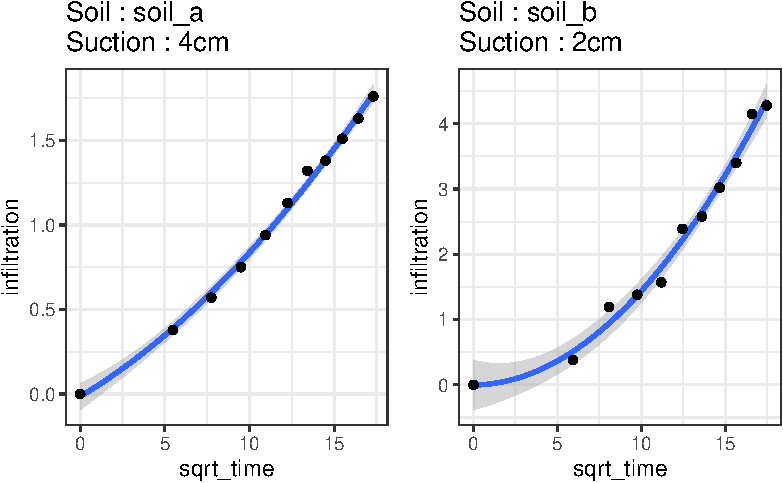
\includegraphics{infiltrodiscR_paper_files/figure-pdf/unnamed-chunk-9-1.pdf}

}

\end{figure}

\hypertarget{conclusions-and-future-work}{%
\subsection{Conclusions and future
work}\label{conclusions-and-future-work}}

The learning curve in R programming and open science practices is not
the same for every researcher, nor is it a dedicated line of research in
graduate programs dedicated to soil physics. Therefore, this experience
in creating an R package homogenizing the data analysis methodology in a
laboratory shows that if there is interest in developing this approach,
further advances in collaboration and reproducibility can be made. Also,
based on the R background of the users of the package, the functions
were developed using the same the grammar, pipelines, and data
visualization practices of tidyverse, which allowed it to be easily
adopted by the researchers.

\hypertarget{acknowledgements}{%
\subsection{Acknowledgements}\label{acknowledgements}}

The authors thank the OLS team for their time and dedication in
motivating researchers to adopt open software practices. Carolina
Giraldo thanks VRI/Faculty of Engineering PUC (Pontificia Universidad
Católica de Chile) Ph.D.~fellowship.Sara Acevedo thanks the research
support provided by CEDEUS (ANID/FONDAP 1522A0002) and the financial
support from Postdoctorado Ingeniería PUC 2023.

\hypertarget{references}{%
\subsection*{References}\label{references}}
\addcontentsline{toc}{subsection}{References}

\hypertarget{refs}{}
\begin{CSLReferences}{1}{0}
\leavevmode\vadjust pre{\hypertarget{ref-https:ux2fux2fdoi.orgux2f10.5281ux2fzenodo.8001894}{}}%
Acevedo, Sara, and Carolina Giraldo. 2023. {``infiltrodiscR: R
Package.''} Zenodo. \url{https://doi.org/10.5281/ZENODO.8001894}.

\leavevmode\vadjust pre{\hypertarget{ref-BondLamberty2016}{}}%
Bond-Lamberty, Ben, A Peyton Smith, and Vanessa Bailey. 2016. {``Running
an Open Experiment: Transparency and Reproducibility in Soil and
Ecosystem Science.''} \emph{Environmental Research Letters} 11 (8):
084004. \url{https://doi.org/10.1088/1748-9326/11/8/084004}.

\leavevmode\vadjust pre{\hypertarget{ref-Carsel1988}{}}%
Carsel, Robert F., and Rudolph S. Parrish. 1988. {``Developing Joint
Probability Distributions of Soil Water Retention Characteristics.''}
\emph{Water Resources Research} 24 (5): 755--69.
\url{https://doi.org/10.1029/wr024i005p00755}.

\leavevmode\vadjust pre{\hypertarget{ref-CORRENDO2023101275}{}}%
Correndo, Adrian A., Austin Pearce, Carl H. Bolster, John T. Spargo,
Deanna Osmond, and Ignacio A. Ciampitti. 2023. {``The Soiltestcorr r
Package: An Accessible Framework for Reproducible Correlation Analysis
of Crop Yield and Soil Test Data.''} \emph{SoftwareX} 21: 101275.
https://doi.org/\url{https://doi.org/10.1016/j.softx.2022.101275}.

\leavevmode\vadjust pre{\hypertarget{ref-vanGenuchten1980}{}}%
Genuchten, M. Th. van. 1980. {``A Closed-Form Equation for Predicting
the Hydraulic Conductivity of Unsaturated Soils.''} \emph{Soil Science
Society of America Journal} 44 (5): 892--98.
\url{https://doi.org/10.2136/sssaj1980.03615995004400050002x}.

\leavevmode\vadjust pre{\hypertarget{ref-Hall2022}{}}%
Hall, Caitlyn A., Sheila M. Saia, Andrea L. Popp, Nilay Dogulu,
Stanislaus J. Schymanski, Niels Drost, Tim van Emmerik, and Rolf Hut.
2022. {``A Hydrologist{\textquotesingle}s Guide to Open Science.''}
\emph{Hydrology and Earth System Sciences} 26 (3): 647--64.
\url{https://doi.org/10.5194/hess-26-647-2022}.

\leavevmode\vadjust pre{\hypertarget{ref-Haynes2023}{}}%
Haynes, Sam. 2023. {``{OLS}: Capacity Building in Open Science with a
Peer-Led, Global, and Diverse Community.''} \emph{Edinburgh Open
Research}, June. \url{https://doi.org/10.2218/eor.2023.8120}.

\leavevmode\vadjust pre{\hypertarget{ref-Lee2019}{}}%
Lee, Sunbok, Suppanut Sriutaisuk, and Hanjoe Kim. 2019. {``Using the
Tidyverse Package in r for Simulation Studies in {SEM}.''}
\emph{Structural Equation Modeling: A Multidisciplinary Journal} 27 (3):
468--82. \url{https://doi.org/10.1080/10705511.2019.1644515}.

\leavevmode\vadjust pre{\hypertarget{ref-METER}{}}%
Meter Group. 2023. \emph{Mini Disk Infiltrometer - Meter Group}.
\url{http://publications.metergroup.com/Manuals/20421_Mini_Disk_Manual_Web.pdf}.

\leavevmode\vadjust pre{\hypertarget{ref-Philip1957THETO}{}}%
Philip, J. R. 1957. {``THE THEORY OF INFILTRATION: 4. SORPTIVITY AND
ALGEBRAIC INFILTRATION EQUATIONS.''} \emph{Soil Science} 84: 257--64.

\leavevmode\vadjust pre{\hypertarget{ref-SoilBiophysics}{}}%
Soil Biophysics Lab. 2023. \emph{Github Account}.
\url{https://github.com/biofisicasuelos}.

\leavevmode\vadjust pre{\hypertarget{ref-10.1016ux2fj.compag.2019.105077}{}}%
Sousa, Decı́ola Fernandes de, Sueli Rodrigues, Herdjania Veras de Lima,
and Lorena Torres Chagas. 2020. {``R Software Packages as a Tool for
Evaluating Soil Physical and Hydraulic Properties.''} \emph{Comput.
Electron. Agric.} 168 (C).
\url{https://doi.org/10.1016/j.compag.2019.105077}.

\leavevmode\vadjust pre{\hypertarget{ref-Surda2019}{}}%
Surda, Peter, Justina Vitkova, Katarina Brezianska, and Lubomir Lichner.
2019. {``Influence of the Infiltration Disk Radius on Determination of
Unsaturated Hydraulic Conductivity of Non-Structural Sandy Soil.''}
\emph{{IOP} Conference Series: Earth and Environmental Science} 221
(March): 012024. \url{https://doi.org/10.1088/1755-1315/221/1/012024}.

\leavevmode\vadjust pre{\hypertarget{ref-Zhang1997}{}}%
Zhang, Renduo. 1997. {``Infiltration Models for the Disk
Infiltrometer.''} \emph{Soil Science Society of America Journal} 61 (6):
1597--1603.
\url{https://doi.org/10.2136/sssaj1997.03615995006100060008x}.

\end{CSLReferences}



\end{document}
